\documentclass{article}\usepackage[]{graphicx}\usepackage[]{color}
% maxwidth is the original width if it is less than linewidth
% otherwise use linewidth (to make sure the graphics do not exceed the margin)
\makeatletter
\def\maxwidth{ %
  \ifdim\Gin@nat@width>\linewidth
    \linewidth
  \else
    \Gin@nat@width
  \fi
}
\makeatother

\definecolor{fgcolor}{rgb}{0.345, 0.345, 0.345}
\newcommand{\hlnum}[1]{\textcolor[rgb]{0.686,0.059,0.569}{#1}}%
\newcommand{\hlstr}[1]{\textcolor[rgb]{0.192,0.494,0.8}{#1}}%
\newcommand{\hlcom}[1]{\textcolor[rgb]{0.678,0.584,0.686}{\textit{#1}}}%
\newcommand{\hlopt}[1]{\textcolor[rgb]{0,0,0}{#1}}%
\newcommand{\hlstd}[1]{\textcolor[rgb]{0.345,0.345,0.345}{#1}}%
\newcommand{\hlkwa}[1]{\textcolor[rgb]{0.161,0.373,0.58}{\textbf{#1}}}%
\newcommand{\hlkwb}[1]{\textcolor[rgb]{0.69,0.353,0.396}{#1}}%
\newcommand{\hlkwc}[1]{\textcolor[rgb]{0.333,0.667,0.333}{#1}}%
\newcommand{\hlkwd}[1]{\textcolor[rgb]{0.737,0.353,0.396}{\textbf{#1}}}%
\let\hlipl\hlkwb

\usepackage{framed}
\makeatletter
\newenvironment{kframe}{%
 \def\at@end@of@kframe{}%
 \ifinner\ifhmode%
  \def\at@end@of@kframe{\end{minipage}}%
  \begin{minipage}{\columnwidth}%
 \fi\fi%
 \def\FrameCommand##1{\hskip\@totalleftmargin \hskip-\fboxsep
 \colorbox{shadecolor}{##1}\hskip-\fboxsep
     % There is no \\@totalrightmargin, so:
     \hskip-\linewidth \hskip-\@totalleftmargin \hskip\columnwidth}%
 \MakeFramed {\advance\hsize-\width
   \@totalleftmargin\z@ \linewidth\hsize
   \@setminipage}}%
 {\par\unskip\endMakeFramed%
 \at@end@of@kframe}
\makeatother

\definecolor{shadecolor}{rgb}{.97, .97, .97}
\definecolor{messagecolor}{rgb}{0, 0, 0}
\definecolor{warningcolor}{rgb}{1, 0, 1}
\definecolor{errorcolor}{rgb}{1, 0, 0}
\newenvironment{knitrout}{}{} % an empty environment to be redefined in TeX

\usepackage{alltt}
\usepackage[hmargin = 1in]{geometry}
\usepackage{enumitem}
\usepackage{amsmath, amsthm, amssymb, amsfonts}
\setlist[2]{
font = \color{black},
before = {\color{red}}
}
\usepackage{textcomp}
\IfFileExists{upquote.sty}{\usepackage{upquote}}{}
\begin{document}





\begin{center} \LARGE
Homework 6
\end{center}
\begin{center} \Large
Due February 27, 2020 at 11:59 PM 
\end{center}



\begin{enumerate}
	\item  Find mean (expected value), median and variance of $X \sim$ Exp($\alpha$). The pdf of Exp($\alpha$) is given by
	\[f(x) = \begin{cases}
	\frac{1}{\alpha} e^{-x/\alpha}&,x > 0\\
	0 &, \mathrm{otherwise} 
	\end{cases}\]
	
	\begin{itemize}
	\item (3 points) Mean:
	
	\begin{align*}
	E(X) & = \int_{0}^\infty x \cdot \frac{1}{\alpha} e^{-x/\alpha} dx\\
	& = \int_{0}^\infty x (- e^{-x/\alpha})' dx\\
	\intertext{Integration by parts:}
	& = - x e^{-x/\alpha} \big|_0^\infty + \int_{0}^\infty e^{-x/\alpha} dx \quad  \\
	& = 0 + ( - \alpha e^{-x/\alpha})\big|_0^\infty\\
	& = \alpha
	\end{align*}
	
	\item (3 points) Variance:
	
		\begin{align*}
	E(X^2) & = \int_{0}^\infty x^2 \cdot \frac{1}{\alpha} e^{-x/\alpha} dx\\
	& = \int_{0}^\infty x^2 (- e^{-x/\alpha})' dx\\
	\intertext{Integration by parts:}
	& = - x^2 e^{-x/\alpha} \big|_0^\infty + \int_{0}^\infty e^{-x/\alpha} \cdot 2x dx \quad  \\
	& = 0 + 2 \alpha \int_{0}^\infty \frac{1}{\alpha} e^{-x/\alpha} dx\\
	& = 2 \alpha^2
	\end{align*}
	Therefore
	\[Var(X) = E(X^2) - (E(X))^2 = 2 \alpha^2 - \alpha^2 = \alpha^2\]
	
	\item (3 points) Median:
	
	\begin{align*}
	& \int_{0}^{Q(0.5)} \frac{1}{\alpha} e^{-x/\alpha} dx = 0.5\\
	\Rightarrow & (-  e^{-x/\alpha})\big|_0^{Q(0.5)} = 1 - e^{-Q(0.5)/\alpha} = 0.5\\
	\Rightarrow & \ln(0.5) = -Q(0.5)/\alpha\\
	\Rightarrow & Q(0.5) = \alpha \ln 2
	\end{align*}
	
	Since $\ln 2 < 1$, we can see the median for exponential distribution is always smaller than the mean.
	\end{itemize}
	
	
	\item P. 263: 5 
	
	\begin{enumerate}
	\item (4 points)
	
	The mean is $\alpha = E(X) = 1000$. The cdf is given by 
	\[F(x) = 1 - e^{-x/1000}.\]
	So the probability that a vehicle of this type gives less than 500 miles of service before first failure is
	\[P(X < 500) = F(500) = 1 - e^{-500/1000} = 0.3934.\]
	The probability that it gives at least 2000 miles of serive before first failure is
	\[P(X \geq 2000) = 1 - F(2000) = e^{-2000/1000} = 0.1353\]
	\item (4 points)
	
	The $q$ quantile $Q(q)$ satisfies
	\[\int_{0}^{Q(q)} f(x) dx = F(Q(q)) = 1 - e^{-Q(q)/1000} = q.\]
	Therefore 
	\[Q(q) = -1000\ln(1 - q).\]
	
	Let $q = 0.05$, $Q(0.05) = -1000 \ln (0.95) = 51.29$.
	
	Let $q = 0.9$, $Q(0.9) = -1000 \ln(0.1) = 2302.58$.
 	\end{enumerate}
	\item P. 329: 31 (3 $\times$ 4 points)
	\begin{enumerate}
	\item (3 points)
	
	$P(X \leq 0.32) = F(0.32) = \sin(0.32) = 0.3146$.
	
	\item (3 points)
	
	$f(x) = \frac{d}{dx}F(x) = \frac{d}{dx} \sin(x) = \cos(x)$ for $0 < x \leq \pi/2$. For $x \leq 0$ or $x > \pi/2$, since the derivative is 0 for a constant, we have $f(x) = \frac{d}{dx} F(x) = 0$.
	
	Therefore
	\[f(x) = \begin{cases}
	\cos(x) & , 0 < x \leq \pi/2\\
	0 &, \mathrm{otherwise}
	\end{cases}\]
	
	\item (3 points)
	
	\begin{align*}
	E(X) & = \int_{0}^{\pi/2} x \cos(x) dx \\
	& = \int_{0}^{\pi/2} x (\sin(x))' dx \\
	\intertext{Integration by parts:}
	& = x \sin(x) \big|_0^{\pi/2} - \int_{0}^{\pi/2} \sin(x) dx\\
	& = \pi/2 - (-\cos(x))\big|_{0}^{\pi/2}\\
	& = \pi/2 - (0 - (-1)) \\
	& = \pi/2 - 1 = 0.5708
	\end{align*}
	
	\item (3 points)
	
	\begin{align*}
	E(X^2) &= \int_{0}^{\pi/2} x^2 \cos (x) dx \\
	& = \int_{0}^{\pi/2} x^2 (\sin(x))'dx\\
	\intertext{Integration by parts:}
	& = x^2 \sin(x)\big|_{0}^{\pi/2} - \int_{0}^{\pi/2} \sin(x) \cdot 2x dx\\
	& = \pi^2/4 - 2 \int_{0}^{\pi/2} x (-\cos(x))' dx\\
	\intertext{Integration by parts:}
	& = \pi^2/4 - 2(-\cos(x) x\big|_{0}^{\pi/2} + \int_{0}^{\pi/2} \cos(x) dx)\\
	& = \pi^2/4 - 2(0 + \sin(x)\big|_0^{\pi/2})\\
	& = \pi^2/4 - 2
	\end{align*}
	Therfore
	\[Var(X) = E(X^2) - (E(X))^2 = \pi^2/4 - 2 - (\pi/2 - 1)^2 = \pi - 3 = 0.1416\]
	\end{enumerate}
	
	\clearpage
	\item P. 332: 41 (6 + 4 + 4 + 7 points)
	\begin{enumerate}
	\item (6 points)
	
	\begin{align*}
	& \int_{-\infty}^\infty f(x) dx = \int_{0}^1 k(x^2(1 - x)) dx = 1\\
	\Rightarrow & k \int_{0}^1 (x^2 - x^3) dx = 1\\
	\Rightarrow & k (\frac{1}{3}x^3 - \frac{1}{4} x^4 )\big|_{0}^1 = 1\\
	\Rightarrow & k (\frac{1}{3} - \frac{1}{4}) = k \frac{1}{12} = 1\\
	\Rightarrow & k = 12
	\end{align*}
	
	
	So the pdf is
	\[f(x) = \begin{cases}
	12x^2(1 - x) & , 0 < x < 1\\
	0 &, \mathrm{otherwise}
	\end{cases}\]
	
\begin{knitrout}
\definecolor{shadecolor}{rgb}{0.969, 0.969, 0.969}\color{fgcolor}

{\centering 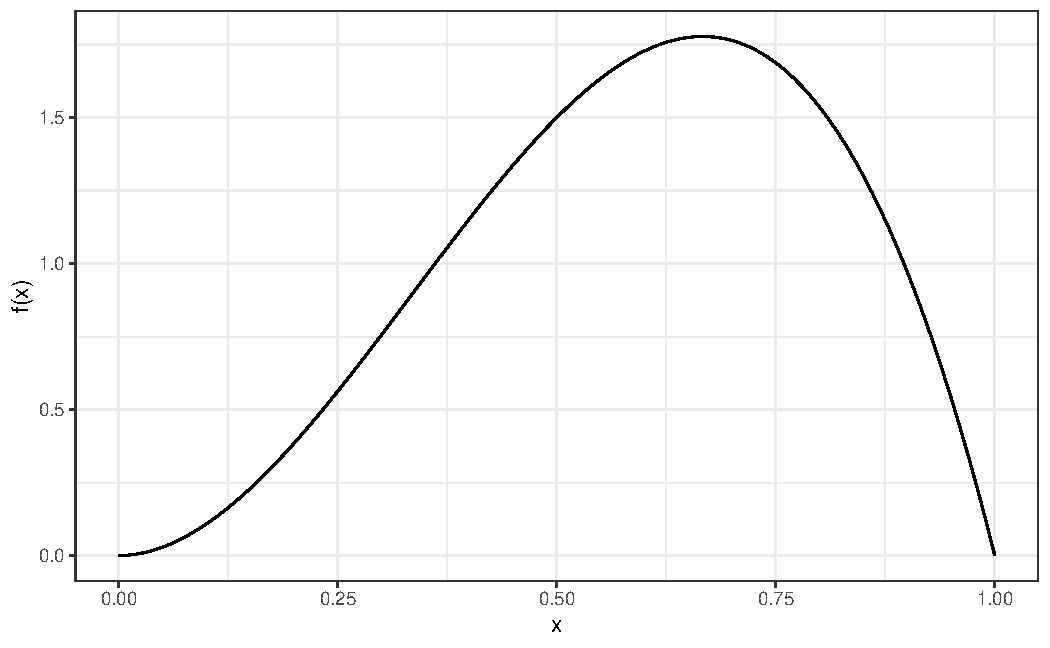
\includegraphics[width=0.6\textwidth]{figure/unnamed-chunk-2-1} 

}



\end{knitrout}
  
  \item (4 points)
  $P(X \leq 0.25) = \int_{0}^{0.25} 12x^2(1 - x) dx = (4x^3 - 3x^4)\big|_{0}^{0.25} = (4(0.25)^3 - 3(0.25)^4) - 0 = 0.0508$.
  
  $P(X \leq 0.75) = \int_{0}^{0.25} 12x^2(1 - x) dx = (4x^3 - 3x^4)\big|_{0}^{0.75} = (4(0.75)^3 - 3(0.75)^4) - 0 = 0.7383$
  
  $P(0.25 < X \leq 0.75) = P(X \leq 0.75) - P(X \leq 0.25) = 0.7383 - 0.0508 = 0.6875$
  
  $P(|X - 0.5| > 0.1) = P(X > 0.5 + 1 \textrm{or} X < 0.5 - 0.1) = P(X > 0.6) + P(X < 0.4) = \int_{0}^{0.4} f(x) dx + \int_{0.6}^1 f(x) dx = 0.7040$
  
  \item (4 points)
  
  \begin{align*}
  E(X) = & \int_{0}^1 x \cdot 12 x^2 (1 - x) dx \\
  =& (3x^4 - \frac{12}{5}x^5)\bigg|_{0}^1 \\
  = & (3 - \frac{12}{5}) - 0\\
  = & \frac{3}{5} = 0.6
  \end{align*}
  
  \begin{align*}
  E(X^2) = & \int_{0}^1 x^2 \cdot 12 x^2 (1 - x) dx \\
  =& (\frac{12}{5} x^5 - 2 x^6)\bigg|_{0}^1 \\
  = & (\frac{12}{5} -2) - 0\\
  = & \frac{2}{5} = 0.4
  \end{align*}
  So
  \[Var(X) = E(X^2) - (E(X))^2 = 0.4 - 0.6^2 = 0.04 \Rightarrow SD(X) = \sqrt{0.04} = 0.2. \]
  
  \item (7 points)
  
  For $x \leq 0$, $F(x) = \int_{-\infty}^x 0 dt = 0$.
  
  For $x \geq 1$, $F(x) = \int_{-\infty}^0 0dt + \int_{0}^1 12t^2(1 - t)dt + \int_{1}^{x} 0dt = 1$.
  
  For $0 < x < 1$, $F(x) = \int_{0}^x 12t^2 (1 - t)dt = 4x^3 - 3x^4.$
  
  So the cdf is
  \[F(x) = \begin{cases}
  0 & , x \leq 0\\
  4x^3 - 3x^4 & , 0 < x  <1\\
  1 &, x \geq 1
  \end{cases}\]
  
\begin{knitrout}
\definecolor{shadecolor}{rgb}{0.969, 0.969, 0.969}\color{fgcolor}

{\centering 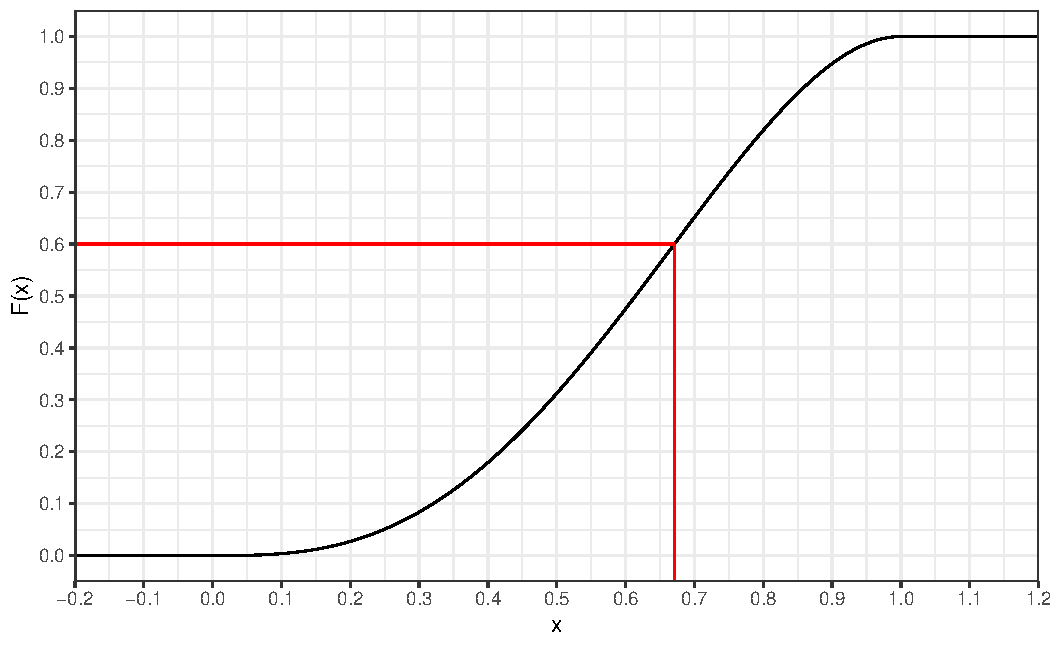
\includegraphics[width=0.6\textwidth]{figure/unnamed-chunk-3-1} 

}



\end{knitrout}
  
  From the plot, we find the 0.6 quantile is around 0.6708.
  	\end{enumerate}
  

\end{enumerate}
%\newpage 
%\nocite{*}
%\bibliographystyle{plainnat} 
%\bibliography{}
\end{document}
